\documentclass{beamer}
\usepackage[utf8]{inputenc}
\usepackage{pgfplots}

\pgfplotsset{compat=1.15}
\usepackage{amsthm}
\usecolortheme{beaver}
\usepackage{pstricks-add}
\pagestyle{empty}
\usepackage{graphicx}

\renewcommand{\qedsymbol}{}
\newtheorem{conjecture}{Conjecture}
\newtheorem{defn}{Definition}
\newtheorem{question}{Question}

\def\arraystretch{1.5}

\title{Trigonometry and a Sequence of Polynomials}
\subtitle{(Chebyshev Polynomials)}
\author{
Andrew Wu\and Jiahua Chen\and Medha Yelimeli\and \\
Siva Muthupalaniappan
\\[12pt] Counselor - Arya Vadnere}
\institute{PROMYS}
\date{2018}


\begin{document}

\frame{\titlepage}

\begin{frame}{Introduction}
 What are Chebyshev polynomials?
 \begin{itemize}
  \item Chebyshev polynomials rewrite $\cos{(nx)}$ into a polynomial or formula in terms of $\cos{(x)}$.
 \end{itemize}
 For example\dots
 \[\cos{(4x)} = 8\cos^4{(x)} - 8 \cos^2{(x)} + 1\]
 We denote the Chebyshev polynomial of $\cos{(nx)}$ as $T_n(\cos{(x)})$, a function on $\cos{(x)}$, and we call this the $n^{th}$ Chebyshev polynomial. From now on, we let $u=\cos{(x)}$. Hence\dots
 \[\cos{(4x)} = T_4(u) = 8u^4 - 8 u^2 + 1\]
\end{frame}

\begin{frame}{The First Few Terms of $T_n$}
 \vspace{-24pt}
 \begin{align*}
  T_0(u) & = 1                                      \\
  T_1(u) & = u                                      \\
  T_2(u) & = 2u^2 - 1                               \\
  T_3(u) & = 4u^3 - 3u                              \\
  T_4(u) & = 8u^4 - 8 u^2 + 1                       \\
  T_5(u) & = 16u^5 - 20u^3 + 5u                     \\
  T_6(u) & = 32u^6 - 48u^4 + 18u^2 - 1              \\
  T_7(u) & = 64u^7 - 112u^5 + 56u^3 - 7u            \\
  T_8(u) & = 128u^8 - 256u^6 + 160u^4 - 32u^2 + 1   \\
  T_9(u) & = 256u^9 - 576u^7 + 432u^5 - 120u^3 + 9u
 \end{align*}
 \center{Any conjectures?}
\end{frame}

\begin{frame}{Noticeable Patterns}
 \vspace{-18pt}
 \tiny{}
 \begin{align*}
  T_0(u) & = \textbf<6>{\textcolor<6>{blue}{1}}                                                                                                                                                                                                                         \\
  T_1(u) & = \textbf<2>{\textcolor<2>{blue}{u}}                                                                                                                                                                                                                         \\
  T_2(u) & = \textbf<2>{\textcolor<2>{blue}{2}} u^{\textbf<4,3>{\textcolor<4,3>{blue}{2}}} - \textbf<6>{\textcolor<6>{blue}{1}}                                                                                                                                         \\
  T_3(u) & = \textbf<2>{\textcolor<2>{blue}{4}} u^{\textbf<4,3>{\textcolor<4,3>{blue}{3}}} - \textbf<5>{\textcolor<5>{blue}{3}} u                                                                                                                                       \\
  T_4(u) & = \textbf<2>{\textcolor<2>{blue}{8}} u^{\textbf<4,3>{\textcolor<4,3>{blue}{4}}} - 8u^{\textbf<4>{\textcolor<4>{blue}{2}}} + \textbf<6>{\textcolor<6>{blue}{1}}                                                                                               \\
  T_5(u) & = \textbf<2>{\textcolor<2>{blue}{16}} u^{\textbf<4,3>{\textcolor<4,3>{blue}{5}}} - 20u^{\textbf<4>{\textcolor<4>{blue}{3}}} + \textbf<5>{\textcolor<5>{blue}{5}} u                                                                                           \\
  T_6(u) & = \textbf<2>{\textcolor<2>{blue}{32}} u^{\textbf<4,3>{\textcolor<4,3>{blue}{6}}} - 48u^{\textbf<4>{\textcolor<4>{blue}{4}}} + 18u^{\textbf<4>{\textcolor<4>{blue}{2}}} - \textbf<6>{\textcolor<6>{blue}{1}}                                                  \\
  T_7(u) & = \textbf<2>{\textcolor<2>{blue}{64}} u^{\textbf<4,3>{\textcolor<4,3>{blue}{7}}} - 112u^{\textbf<4>{\textcolor<4>{blue}{5}}} + 56u^{\textbf<4>{\textcolor<4>{blue}{3}}} - \textbf<5>{\textcolor<5>{blue}{7}} u                                               \\
  T_8(u) & = \textbf<2>{\textcolor<2>{blue}{128}} u^{\textbf<4,3>{\textcolor<4,3>{blue}{8}}} - 256u^{\textbf<4>{\textcolor<4>{blue}{6}}} + 160u^{\textbf<4>{\textcolor<4>{blue}{4}}} - 32u^{\textbf<4>{\textcolor<4>{blue}{2}}} + \textbf<6>{\textcolor<6>{blue}{1}}    \\
  T_9(u) & = \textbf<2>{\textcolor<2>{blue}{256}} u^{\textbf<4,3>{\textcolor<4,3>{blue}{9}}} - 576u^{\textbf<4>{\textcolor<4>{blue}{7}}} + 432u^{\textbf<4>{\textcolor<4>{blue}{5}}} - 120u^{\textbf<4>{\textcolor<4>{blue}{3}}} + \textbf<5>{\textcolor<5>{blue}{9}} u
 \end{align*} \normalsize
 \vspace{-15pt}
 \hline
 \begin{itemize}
  \pause
  \item Leading coefficients are powers of 2. \pause
  \item $T_n$ is of degree $n$. \pause
  \item Powers of $u$ are either even or odd, never both. \pause
  \item For odd $n$, the ending coefficients are $\pm n$ \pause
  \item For even $n$, the ending coefficients are $\pm 1$ \pause
  \item Terms are alternating.
 \end{itemize}
\end{frame}

\begin{frame}{Some More Patterns}
 \vspace{-18pt}
 \tiny{}
 \begin{align*}
  T_0(u) & = 1                                                                                                                                            \\
  T_1(u) & = u                                                                                                                                            \\
  T_2(u) & = \textbf<4>{\textcolor<4>{blue}{2}} u^2 - \textbf<3,6>{\textcolor<3,6>{blue}{1}}                                                              \\
  T_3(u) & = \textbf<5>{\textcolor<5>{blue}{4}} u^3 - \textbf<3,6>{\textcolor<3,6>{blue}{3}} u                                                            \\
  T_4(u) & = 8u^4 - \textbf<3,4,6>{\textcolor<3,4,6>{blue}{8}} u^2 + 1                                                                                    \\
  T_5(u) & = 16u^5 - \textbf<3,5,6>{\textcolor<3,5,6>{blue}{20}} u^3 + \textbf<6>{\textcolor<6>{blue}{5}}u                                                \\
  T_6(u) & = 32u^6 - \textbf<3,6>{\textcolor<3,6>{blue}{48}} u^4 + \textbf<4,6>{\textcolor<4,6>{blue}{18}} u^2 - 1                                        \\
  T_7(u) & = 64u^7 - \textbf<3>{\textcolor<3>{blue}{112}} u^5 + \textbf<5,6>{\textcolor<5,6>{blue}{56}}u^3 - 7u                                           \\
  T_8(u) & = 128u^8 - \textbf<3>{\textcolor<3>{blue}{256}} u^6 + \textbf<6>{\textcolor<6>{blue}{160}} u^4 - \textbf<4>{\textcolor<4>{blue}{32}} u^2 + 1   \\
  T_9(u) & = 256u^9 - \textbf<3>{\textcolor<3>{blue}{576}} u^7 + \textbf<6>{\textcolor<6>{blue}{432}} u^5 - \textbf<5>{\textcolor<5>{blue}{120}} u^3 + 9u
 \end{align*} \normalsize
 \vspace{-15pt}
 \hline
 \begin{itemize}
  \pause
  \item $T_n(1)=1$ (in other words, coefficients sum to 1). \pause
  \item The 2nd term has coefficient $-2^{n-3}\cdot n$ \pause
  \item The coefficient of the $u^2$ term for $T_{2k}$ is $\pm 2k^2$ \pause
  \item The coefficient of the $u^3$ term for $T_{2k-1}$ is $\pm \binom{2k}{3}$ \pause
  \item The coefficient of the $u^{n-4}$ in $T_n$ is $n\cdot s$, where $-s$ is the coefficient of the $u^{n-5}$ in $T_{n-3}$.
 \end{itemize}
\end{frame}

\begin{frame}{Recursive Formula}
 \vspace{-18pt}
 \tiny{}
 \begin{align*}
  T_0(u) & = 1                                      \\
  T_1(u) & = u                                      \\
  T_2(u) & = 2u^2 - 1                               \\
  T_3(u) & = 4u^3 - 3u                              \\
  T_4(u) & = 8u^4 - 8 u^2 + 1                       \\
  T_5(u) & = 16u^5 - 20u^3 + 5u                     \\
  T_6(u) & = 32u^6 - 48u^4 + 18u^2 - 1              \\
  T_7(u) & = 64u^7 - 112u^5 + 56u^3 - 7u            \\
  T_8(u) & = 128u^8 - 256u^6 + 160u^4 - 32u^2 + 1   \\
  T_9(u) & = 256u^9 - 576u^7 + 432u^5 - 120u^3 + 9u
 \end{align*} \normalsize
 \hline
 \vspace{12pt}
 \begin{conjecture}\center
  \vspace{-12pt}
  $T_n(u)=2u\cdot T_{n-1}(u)-T_{n-2}(u)$
 \end{conjecture}
\end{frame}

\begin{frame}{Proof of Recursive Formula}
 \begin{conjecture}\center
  \vspace{-12pt}
  $T_n(u)=2u\cdot T_{n-1}(u)-T_{n-2}(u)$
 \end{conjecture}
 \pause
 \begin{proof}
  Recall that\dots
  \begin{align*}
   \cos{(a+b)}         & =\cos{(a)}\cos{(b)}-\sin{(a)}\sin{(b)}   \\
   \intertext{What we want is $\cos{(nx)}$ expressed using previous terms, so we let $a=(n-1)x$ and $b=x$ and thus $a+b=nx$}
   \cos ((n-1)x+x)     & =\cos((n-1)x)\cos(x)-\sin((n-1)x)\sin(x) \\[12pt]
   \sin((n-1)x)\sin(x) & =\cos((n-1)x)\cos(x) - \cos ((n-1)x+x)
  \end{align*}
 \end{proof}
\end{frame}

\begin{frame}{Proof of Recursive Formula}
 Using the product-to-sum formula for $\sin(a)\sin(b)$, we get\dots
 \begin{align*}
  \sin(nx-x)\sin(x)               & =\cos((n-1)x)\cos(x) - \cos ((n-1)x+x)                     \\[12pt]
  \frac{\cos(nx-2x) -\cos(nx)}{2} & =\cos((n-1)x)\cos(x) - \cos ((n-1)x+x)                     \\[12pt]
  \cos(nx-2x) -\cos(nx)           & = 2\cos((n-1)x)\cos(x) - 2\cos (nx)                        \\[12pt]
  \cos(nx)                        & = 2\cos((n-1)x)\cos(x) - \cos((n-2)x)                      \\[12pt]
  T_n(u)                          & = 2T_{n-1}(u)\cdot u - T_{n-2}(u)      \qquad \blacksquare
 \end{align*}
\end{frame}


\begin{frame}{General Formula}
 \vspace{-18pt}
 \tiny{}
 \begin{align*}
  T_0(u) & = 1                                      \\
  T_1(u) & = u                                      \\
  T_2(u) & = 2u^2 - 1                               \\
  T_3(u) & = 4u^3 - 3u                              \\
  T_4(u) & = 8u^4 - 8 u^2 + 1                       \\
  T_5(u) & = 16u^5 - 20u^3 + 5u                     \\
  T_6(u) & = 32u^6 - 48u^4 + 18u^2 - 1              \\
  T_7(u) & = 64u^7 - 112u^5 + 56u^3 - 7u            \\
  T_8(u) & = 128u^8 - 256u^6 + 160u^4 - 32u^2 + 1   \\
  T_9(u) & = 256u^9 - 576u^7 + 432u^5 - 120u^3 + 9u
 \end{align*} \normalsize
 \hline
 \vspace{12pt}
 \begin{conjecture}\center
  \vspace{-12pt}
  $T_n(u) = \displaystyle\sum_{k=0}^{\left\lfloor \tfrac{n}{2} \right\rfloor} \left[(u^2-1)^k \cdot u^{n-2k} \cdot \binom{n}{2k}\right]$
 \end{conjecture}
\end{frame}

\begin{frame}{Computing $T_5(u)$ with the General Formula}
 \vspace{-12pt}
 \[T_n(u) = \displaystyle\sum_{k=0}^{\left\lfloor \tfrac{n}{2} \right\rfloor} \left[(u^2-1)^k \cdot u^{n-2k} \cdot \binom{n}{2k}\right]\] \pause
 \[T_5(u) = \displaystyle\sum_{k=0}^{2} \left[(u^2-1)^k \cdot u^{5-2k} \cdot \binom{5}{2k}\right]\] \pause
 \[k=0 : \left[(u^2-1)^0 \cdot u^{5-2\cdot 0} \cdot \binom{5}{2\cdot 0}\right]=u^5\] \pause
 \[k=1 : \left[(u^2-1)^1 \cdot u^{5-2\cdot 1} \cdot \binom{5}{2\cdot 1}\right]=10u^5-10u^3\] \pause
 \[k=2 : \left[(u^2-1)^2 \cdot u^{5-2\cdot 2} \cdot \binom{5}{2\cdot 2}\right]=5u^5-10u^3+5u\] \pause
 \[T_5(u)=16u^5-20u^3+5u\]
\end{frame}

\begin{frame}{General Formula \#2}
 \vspace{-18pt}
 \tiny{}
 \begin{align*}
  T_0(u) & = 1                                      \\
  T_1(u) & = u                                      \\
  T_2(u) & = 2u^2 - 1                               \\
  T_3(u) & = 4u^3 - 3u                              \\
  T_4(u) & = 8u^4 - 8 u^2 + 1                       \\
  T_5(u) & = 16u^5 - 20u^3 + 5u                     \\
  T_6(u) & = 32u^6 - 48u^4 + 18u^2 - 1              \\
  T_7(u) & = 64u^7 - 112u^5 + 56u^3 - 7u            \\
  T_8(u) & = 128u^8 - 256u^6 + 160u^4 - 32u^2 + 1   \\
  T_9(u) & = 256u^9 - 576u^7 + 432u^5 - 120u^3 + 9u
 \end{align*} \normalsize
 \hline
 \vspace{12pt}
 \begin{conjecture}\center
  \vspace{-12pt}
  $T_{n}(u) = \frac{1}{2} \left[ \frac{1}{(u+\sqrt{u^{2}-1})^{n}} + \frac{1}{(u-\sqrt{u^{2}-1})^{n}} \right]$
 \end{conjecture}
\end{frame}

\begin{frame}{Explaining General Formula \#2}
 \begin{conjecture}\center
  \vspace{-12pt}
  $T_{n}(u) = \frac{1}{2} \left[ \frac{1}{(u+\sqrt{u^{2}-1})^{n}} + \frac{1}{(u-\sqrt{u^{2}-1})^{n}} \right]$ \\[12pt]
 \end{conjecture}
 \pause
 \begin{proof}
 We define a generating function for $T_n(u)$\dots
 \[\text{Let } f(x) = \displaystyle \sum_{n=0}^{\infty} T_{n}x^{n}.\]
 We use our recursive formula and multiply $f(x)$ by $2u$, then consider $2ux f(x) - f(x)$.
 \end{proof}
\end{frame}

\begin{frame}{Explaining General Formula \#2}
Stuff cancels! We get
$$f(x) = \frac{1-ux}{1 - 2ux + x^2}.$$
We then use partial fractions, letting be $p$ and $q$ be the roots of the quadratic $1 - 2ux + x^2$:
$$\dfrac{A}{x-p} + \dfrac{B}{x-q} = \dfrac{1 - ux}{1 - 2ux + x^2}.$$
If we make the substitution $A' = -Ap$ and $B' = -Bq$, then we can instead solve
$$A'\cdot \left( \dfrac{1}{1 - \frac{x}{p}} \right)+ B' \cdot \left( \dfrac{1}{1- \frac{x}{q}} \right) = \dfrac{1 - ux}{1 - 2ux + x^2} = f(x).$$
We can rewrite the LHS with geometric series and equate coefficients!
\end{frame}

\begin{frame}{Explaining General Formula \#2}
It follows that
$$A' \cdot \left( \frac{1}{p} \right)^k + B' \cdot \left( \frac{1}{q} \right)^k = T_k.$$
We set $k = 0$ and $k = 1$ to give us equations. We can express $p$ and $q$ in terms of $u$ using the quadratic formula: recall that $(x-p)(x-q) = 1 - 2ux + x^2$, so $p = u + \sqrt{u^2 - 1}, q = u - \sqrt{u^2 - 1}$. After some work, we get $A' = B' = \frac{1}{2}$, so our general formula becomes
$$T_{n}(u) = \frac{1}{2} \left[ \frac{1}{(u+\sqrt{u^{2}-1})^{n}} + \frac{1}{(u-\sqrt{u^{2}-1})^{n}} \right]$$

\end{frame}

\begin{frame}{Exploring Graphs of $T_n$}
 \vspace{-12pt}
 \center{What happens when we look at the graph of $T_n(u)$?}
 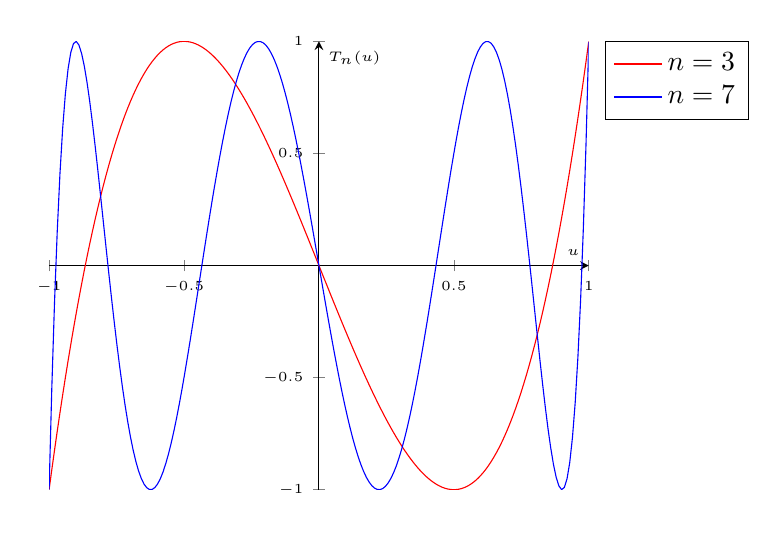
\begin{tikzpicture}
  \begin{axis}[
    axis lines = middle,
    xlabel = $u$,
    ylabel = {$T_n(u)$},
    label style={font=\tiny},
    tick label style={font=\tiny},
    legend pos=outer north east,
   ]
   \addplot [
    domain=-1:1,
    samples=200,
    color=red,
   ]
   {4*x^3 - 3*x};
   \addlegendentry{$n=3$}
   \addplot [
    domain=-1:1,
    samples=200,
    color=blue,
   ]
   {64*x^7 - 112*x^5 + 56*x^3 - 7*x};
   \addlegendentry{$n=7$}

  \end{axis}
 \end{tikzpicture}
\end{frame}

\begin{frame}{The First Few Graphs of $T_n$}
 \vspace{-12pt}
 \[T_1(u)=u\]
 \center{
  \begin{tikzpicture}
   \begin{axis}[
     axis lines = middle,
     xlabel = $u$,
     ylabel = {$T_n(u)$},
     label style={font=\tiny},
     tick label style={font=\tiny},
    ]
    \addplot [
     domain=-1:1,
     samples=200,
     color=blue,
    ]
    {x};
   \end{axis}
  \end{tikzpicture}}
\end{frame}


\begin{frame}{The First Few Graphs of $T_n$}
 \vspace{-12pt}
 \[T_2(u)=2u^2-1\]
 \center{
  \begin{tikzpicture}
   \begin{axis}[
     axis lines = middle,
     xlabel = $u$,
     ylabel = {$T_n(u)$},
     label style={font=\tiny},
     tick label style={font=\tiny},
    ]
    \addplot [
     domain=-1:1,
     samples=200,
     color=blue,
    ]
    {2*x^2-1};
   \end{axis}
  \end{tikzpicture}}
\end{frame}

\begin{frame}{The First Few Graphs of $T_n$}
 \vspace{-12pt}
 \[T_3(u) = 4u^3 - 3u\]
 \center{
  \begin{tikzpicture}
   \begin{axis}[
     axis lines = middle,
     xlabel = $u$,
     ylabel = {$T_n(u)$},
     label style={font=\tiny},
     tick label style={font=\tiny},
    ]
    \addplot [
     domain=-1:1,
     samples=200,
     color=blue,
    ]
    {4*x^3-3*x};
   \end{axis}
  \end{tikzpicture}}
\end{frame}

\begin{frame}{The First Few Graphs of $T_n$}
 \vspace{-12pt}
 \[T_4(u) = 8u^4 - 8u^2 + 1\]
 \center{
  \begin{tikzpicture}
   \begin{axis}[
     axis lines = middle,
     xlabel = $u$,
     ylabel = {$T_n(u)$},
     label style={font=\tiny},
     tick label style={font=\tiny},
    ]
    \addplot [
     domain=-1:1,
     samples=200,
     color=blue,
    ]
    {8*x^4-8*x^2+1};
   \end{axis}
  \end{tikzpicture}}
\end{frame}

\begin{frame}{The First Few Graphs of $T_n$}
 \vspace{-12pt}
 \[T_5(u) = 16u^5 - 20u^3 + 5u\]
 \center{
  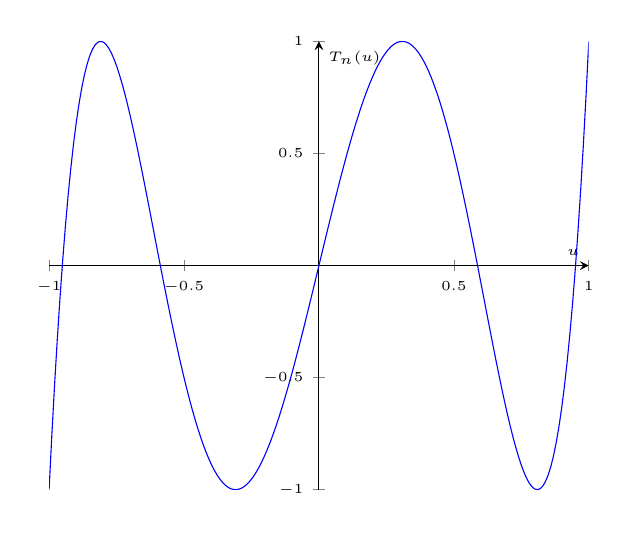
\begin{tikzpicture}
   \begin{axis}[
     axis lines = middle,
     xlabel = $u$,
     ylabel = {$T_n(u)$},
     label style={font=\tiny},
     tick label style={font=\tiny},
    ]
    \addplot [
     domain=-1:1,
     samples=200,
     color=blue,
    ]
    {16*x^5-20*x^3+5*x};
   \end{axis}
  \end{tikzpicture}}
\end{frame}

\begin{frame}{Initial Observations of Graphs of $T_n$}
 \center{$T_n(u)$ is an even function $\iff$ $n$ is even} \\
 \center{$T_n(u)$ is an odd function $\iff$ $n$ is odd} \\
\end{frame}

\begin{frame}{An Interesting Observation}
 \vspace{-12pt}
 \[T_1(u), T_2(u), T_3(u), T_4(u), T_5(u), T_6(u), T_7(u), T_8(u)\]
 \center{
  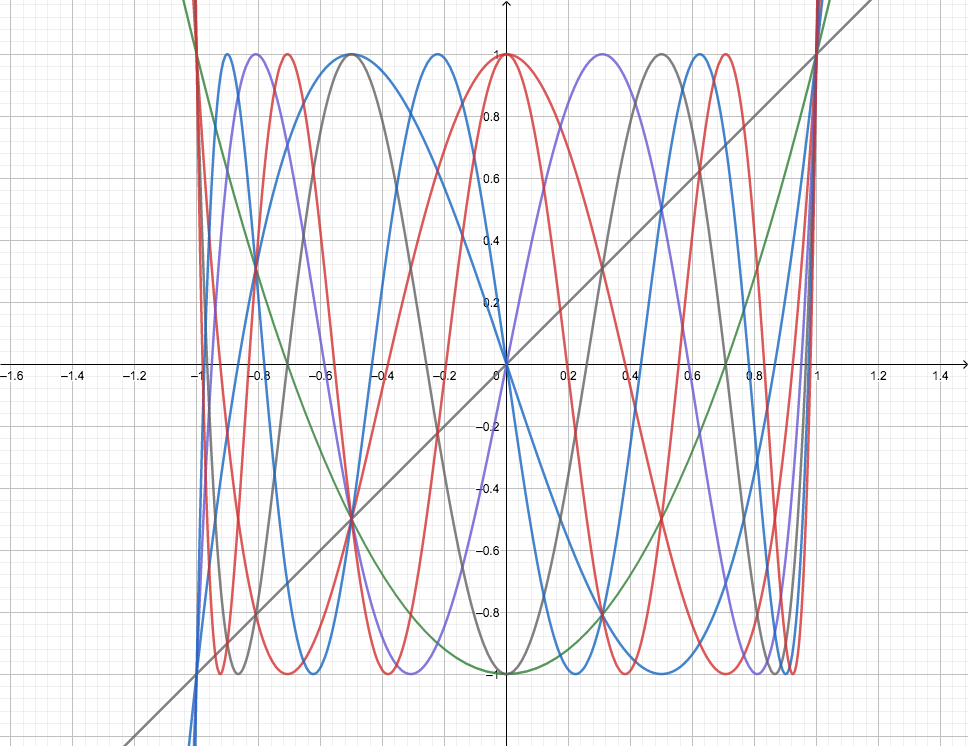
\includegraphics[scale=.26]{pic2.png}
 }
\end{frame}

\begin{frame}{Intersection $(-0.5,-0.5)$}
 \vspace{-12pt}
 \[T_1(u), T_2(u), T_4(u), T_5(u), T_7(u), T_8(u)\qquad (3\nmid n)\]
 \center{
  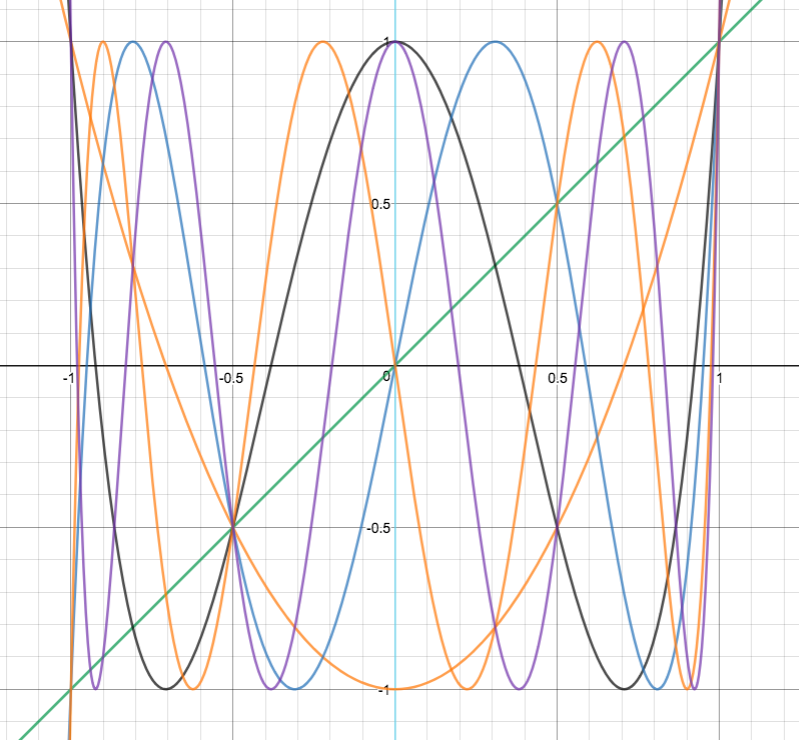
\includegraphics[scale=.26]{pic3.png}
 }
\end{frame}

\begin{frame}{Explaining $(-0.5,-0.5)$}
 \begin{conjecture}\center
  \vspace{-12pt}
  $n\in\mathbb{N} \land 3\nmid n \implies T_n(-0.5)=-0.5$ \\
  In other words, $T_n(u)$ passes through point $(-0.5,-0.5)$ \\[12pt]
 \end{conjecture}
 \pause
 \begin{proof}
  \vspace{-12pt}
  \[3\nmid n\implies n=3k\pm 1\] \pause
  \vspace{-12pt}
  \[T_n(u)=T_{3k\pm 1}(\cos{x})=\cos{((3k\pm 1)x)}\] \pause
  \vspace{-12pt}
  \[\cos^{-1}(-\frac{1}{2})=\pm\frac{2\pi}{3}\] \pause
  \vspace{-6pt}
  \[T_{3k\pm 1}(-\frac{1}{2})=T_{3k\pm 1}\left(\cos{\left(\pm \frac{2\pi}{3}\right)}\right)=\cos{\left((3k\pm 1)\left(\pm\frac{2\pi}{3}\right)\right)}\]\pause
  \vspace{-6pt}
  \[=\cos{\left(\pm 2k\pi\pm \frac{2\pi}{3}\right)}=\cos{\left(\pm \frac{2\pi}{3}\right)}=-0.5\qquad \blacksquare\]
  \vspace{6pt}
 \end{proof}
\end{frame}

\begin{frame}{Intersection $(-0.5,1)$}
 \vspace{-12pt}
 \[T_3(u), T_6(u), T_9(u)\qquad (3| n)\]
 \center{
  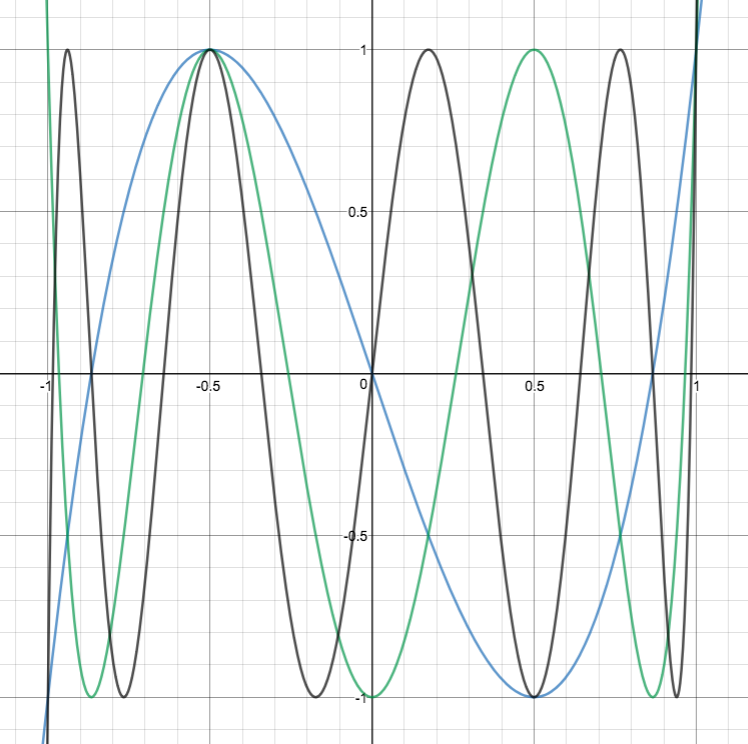
\includegraphics[scale=.26]{pic4.png}
 }
\end{frame}

\begin{frame}{Explaining $(-0.5,1)$}
 \begin{conjecture}\center
  \vspace{-12pt}
  $n\in\mathbb{N}, T_{3n}(-0.5)=1$ \\
  In other words, $T_{3n}(u)$ passes through point $(-0.5,1)$ \\[12pt]
 \end{conjecture}
 \pause
 \begin{proof}
  \vspace{-12pt}
  \[T_{3n}(-0.5)=\cos\left(3n\cdot \pm \frac{2\pi}{3}\right)=\cos(\pm 2n\cdot \pi)=1\qquad \blacksquare\]
 \end{proof}
\end{frame}

\begin{frame}{Intersections of $T_n(u)$ and $T_m(u)$}
 \begin{definition}
  We define $I(n,m)$ as the number of intersections of the graphs of $T_n(u)$ and $T_m(u)$. In other words, the number of solutions to $T_n(u)=T_m(u)$.
 \end{definition}
 \vspace{24pt}
 \begin{question}
  Can we predict $I(n,m)$ given $n,m$?
 \end{question}
\end{frame}

\begin{frame}{Some Numerical Examples of $I(n,m)$}
 \vspace{-12pt}
 \[I(2,3)=3\]
 \center{
  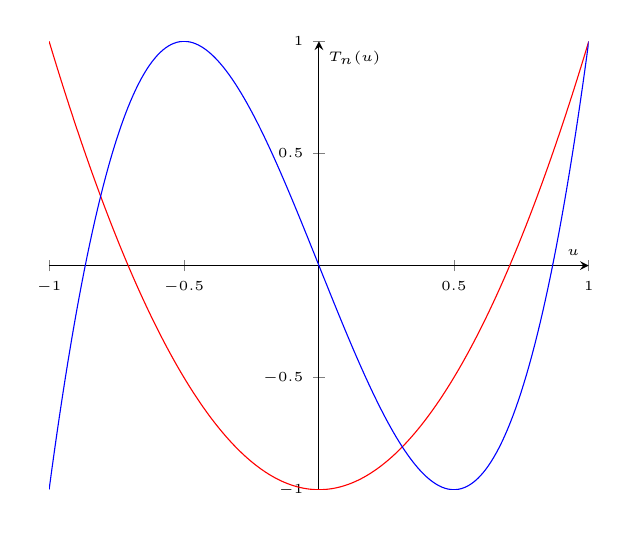
\begin{tikzpicture}
   \begin{axis}[
     axis lines = middle,
     xlabel = $u$,
     ylabel = {$T_n(u)$},
     label style={font=\tiny},
     tick label style={font=\tiny},
    ]
    \addplot [
     domain=-1:1,
     samples=200,
     color=red,
    ]
    {2*x^2 - 1};
    \addplot [
     domain=-1:1,
     samples=200,
     color=blue,
    ]
    {4*x^3 - 3*x};

   \end{axis}
  \end{tikzpicture}}
\end{frame}

\begin{frame}{Some Numerical Examples of $I(n,m)$}
 \vspace{-12pt}
 \[I(2,4)=4\]
 \center{
  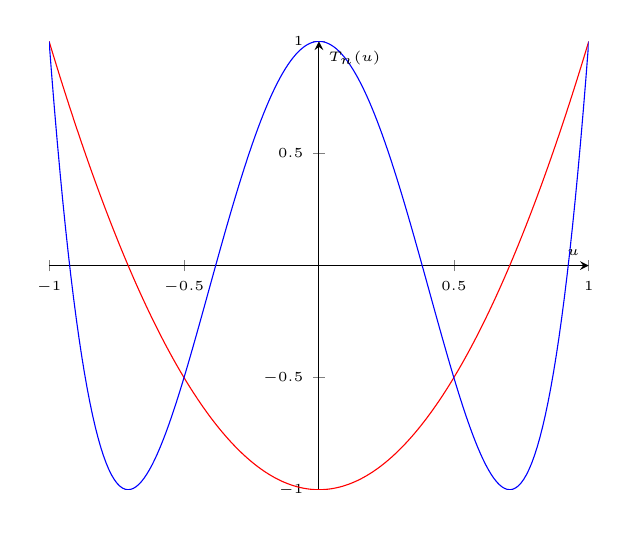
\begin{tikzpicture}
   \begin{axis}[
     axis lines = middle,
     xlabel = $u$,
     ylabel = {$T_n(u)$},
     label style={font=\tiny},
     tick label style={font=\tiny},
    ]
    \addplot [
     domain=-1:1,
     samples=200,
     color=red,
    ]
    {2*x^2 - 1};
    \addplot [
     domain=-1:1,
     samples=200,
     color=blue,
    ]
    {8*x^4-8*x^2+1};

   \end{axis}
  \end{tikzpicture}}
\end{frame}

\begin{frame}{Some Numerical Examples of $I(n,m)$}
 \vspace{-12pt}
 \[I(4,5)=5\]
 \center{
  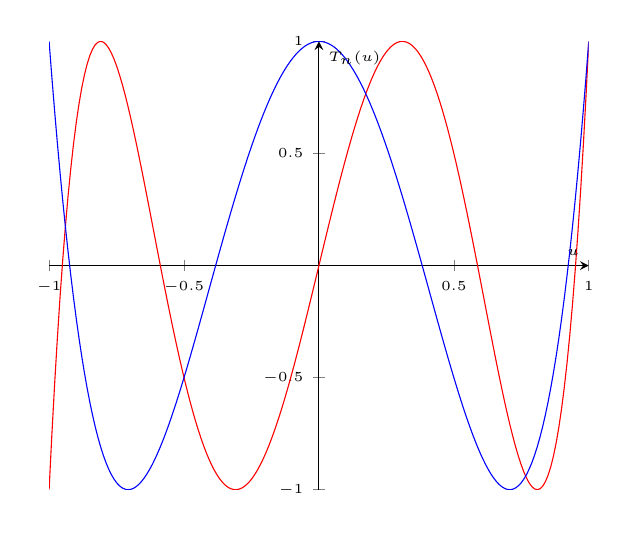
\begin{tikzpicture}
   \begin{axis}[
     axis lines = middle,
     xlabel = $u$,
     ylabel = {$T_n(u)$},
     label style={font=\tiny},
     tick label style={font=\tiny},
    ]
    \addplot [
     domain=-1:1,
     samples=200,
     color=red,
    ]
    {16*x^5-20*x^3+5*x};
    \addplot [
     domain=-1:1,
     samples=200,
     color=blue,
    ]
    {8*x^4-8*x^2+1};

   \end{axis}
  \end{tikzpicture}}
\end{frame}

\begin{frame}{Some Numerical Examples of $I(n,m)$}
 \vspace{-12pt}
 \[I(4,7)=7\]
 \center{
  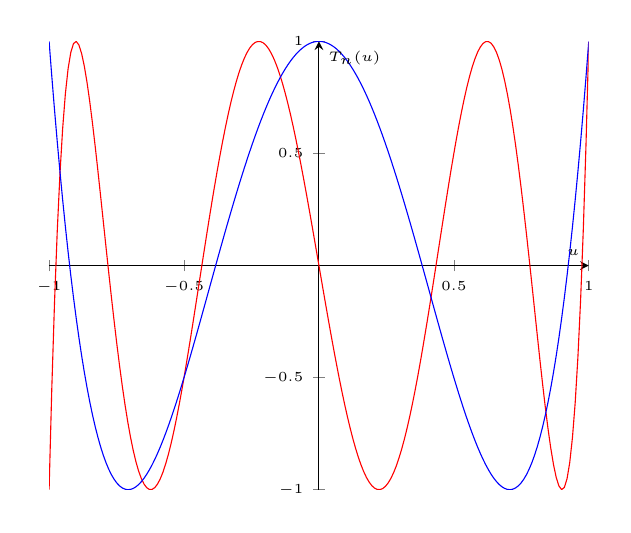
\begin{tikzpicture}
   \begin{axis}[
     axis lines = middle,
     xlabel = $u$,
     ylabel = {$T_n(u)$},
     label style={font=\tiny},
     tick label style={font=\tiny},
    ]
    \addplot [
     domain=-1:1,
     samples=200,
     color=red,
    ]
    {64*x^7-112*x^5+56*x^3-7*x};
    \addplot [
     domain=-1:1,
     samples=200,
     color=blue,
    ]
    {8*x^4-8*x^2+1};

   \end{axis}
  \end{tikzpicture}}
\end{frame}

\begin{frame}{Some Numerical Examples of $I(n,m)$}
 \vspace{-12pt}
 \[I(4,8)=7\]
 \center{
  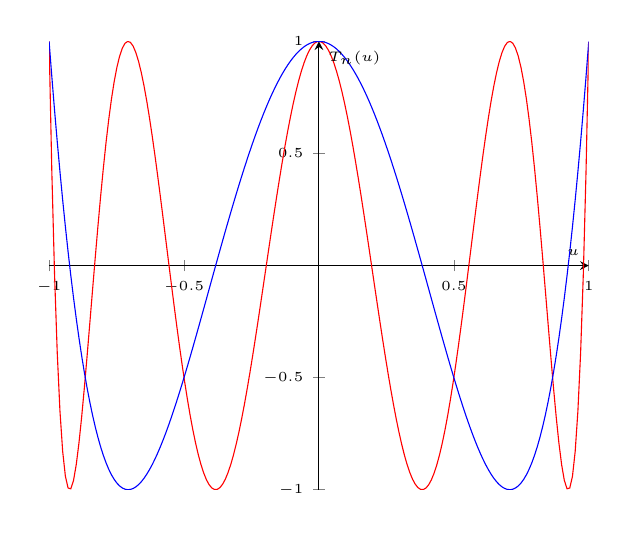
\begin{tikzpicture}
   \begin{axis}[
     axis lines = middle,
     xlabel = $u$,
     ylabel = {$T_n(u)$},
     label style={font=\tiny},
     tick label style={font=\tiny},
    ]
    \addplot [
     domain=-1:1,
     samples=200,
     color=red,
    ]
    {128*x^8-256*x^6+160*x^4-32*x^2+1};
    \addplot [
     domain=-1:1,
     samples=200,
     color=blue,
    ]
    {8*x^4-8*x^2+1};

   \end{axis}
  \end{tikzpicture}}
\end{frame}

\begin{frame}{Some Numerical Examples of $I(n,m)$}
 \vspace{-12pt}
 \[I(7,8)=8\]
 \center{
  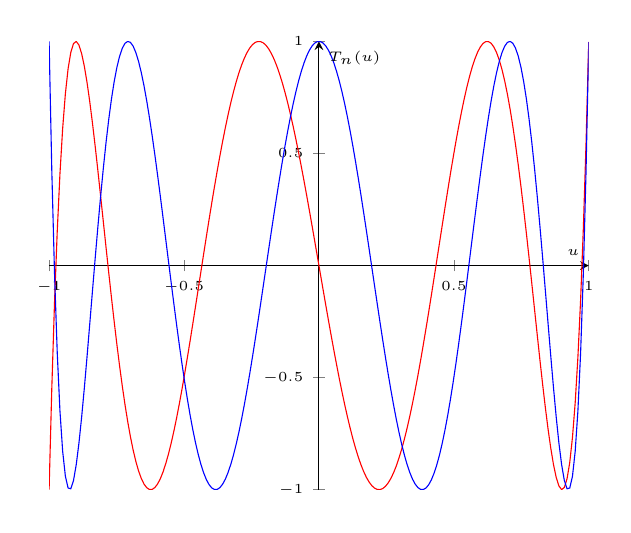
\begin{tikzpicture}
   \begin{axis}[
     axis lines = middle,
     xlabel = $u$,
     ylabel = {$T_n(u)$},
     label style={font=\tiny},
     tick label style={font=\tiny},
    ]
    \addplot [
     domain=-1:1,
     samples=200,
     color=red,
    ]
    {64*x^7-112*x^5+56*x^3-7*x};
    \addplot [
     domain=-1:1,
     samples=200,
     color=blue,
    ]
    {128*x^8-256*x^6+160*x^4-32*x^2+1};

   \end{axis}
  \end{tikzpicture}}
\end{frame}

\begin{frame}{Some Numerical Examples of $I(n,m)$}
 \begin{table}[]
  \begin{tabular}{r|c|c|c|c|c|ccc|c|c|c}
   $n$      & $2$ & $2$ & $4$ & $4$ & $4$ & $7$ &          & $2$  & $10$ & $5$  & $3$ \\ \hline
   $m$      & $3$ & $4$ & $5$ & $7$ & $8$ & $8$ & $\cdots$ & $10$ & $12$ & $10$ & $9$ \\ \hline
   $I(n,m)$ & $3$ & $4$ & $5$ & $7$ & $7$ & $8$ &          & $9$  & $12$ & $8$  & $7$ \\
  \end{tabular}
 \end{table}
\end{frame}

\begin{frame}{$T_n(u)$ in $\mathbb{Z}_p[u]$}
 \vspace{-6pt}
 \begin{question}
  What \textbf{structures} do the coefficients of $T_n(u)$ exhibit modulo prime $p$? (In other words, what do we get when we observe the coefficients of $T_n(u)$ in $\mathbb{Z}_p[u]$?)
 \end{question}
 \vspace{12pt} \pause
 First, we want to `equate' several different terms so we can easily compare them and discover patterns. Hence, we first add in the zero coefficients. \pause
 \[T_5(u) = 16u^5 - 20u^3 + 5u\] \pause
 \[=16u^5 + 0u^4- 20u^3 +0u^2 + 5u + 0\] \pause
 Then, we reverse the ordering of the polynomial, so that the $u^0$ term comes first. \pause
 \[T_5(u)=0+5u +0u^2 - 20u^3  + 0u^4+ 16u^5\]
\end{frame}

\begin{frame}{$T_n(u)$ in $\mathbb{Z}_p[u]$}
 \vspace{-6pt}
 \center{which all yields\dots}
 \begin{align*}
  T_0(u) & = 1                                         \\
  T_1(u) & = 0+u                                       \\
  T_2(u) & = -1 + 0u + 2u^2                            \\
  T_3(u) & = 0 -3u +0u^2 + 4u^3                        \\
  T_4(u) & = 1+0u-8u^2+0u^3+  8u^4                     \\
  T_5(u) & = 0+5u+0u^2-20u^3+0u^4+ 16u^5               \\
  T_6(u) & = -1 + 0u + 18u^2+0u^3 -48u^4 +0u^5 + 32u^6
 \end{align*}
 \center{\dots}
\end{frame}

\begin{frame}{$T_n(u)$ in $\mathbb{Z}_p[u]$}
 \vspace{-6pt}
 \center{Now, since the coefficient terms are now matching, we extrapolate the coefficients and place them into a table\dots }
 \begin{table}[]
  \begin{tabular}{|c|c|c|c|c|c|c|c|}
   \hline
   \multicolumn{1}{|l|}{$n$} & \multicolumn{1}{l|}{$u^0$} & \multicolumn{1}{l|}{$u^1$} & \multicolumn{1}{l|}{$u^2$} & \multicolumn{1}{l|}{$u^3$} & \multicolumn{1}{l|}{$u^4$} & \multicolumn{1}{l|}{$u^5$} & \multicolumn{1}{l|}{$u^6$} \\ \hline
   0                         & 1                          &                            &                            &                            &                            &                            &                            \\ \hline
   1                         & 0                          & 1                          &                            &                            &                            &                            &                            \\ \hline
   2                         & -1                         & 0                          & 2                          &                            &                            &                            &                            \\ \hline
   3                         & 0                          & -3                         & 0                          & 4                          &                            &                            &                            \\ \hline
   4                         & 1                          & 0                          & -8                         & 0                          & 8                          &                            &                            \\ \hline
   5                         & 0                          & 5                          & 0                          & -20                        & 0                          & 16                         &                            \\ \hline
   6                         & -1                         & 0                          & 18                         & 0                          & -48                        & 0                          & 32                         \\ \hline
  \end{tabular}
 \end{table}
\end{frame}

\begin{frame}{$T_n(u)$ in $\mathbb{Z}_p[u]$}
 \vspace{-6pt}
 \center{Taken mod $7$\dots }
 \begin{table}[]
  \begin{tabular}{|c|c|c|c|c|c|c|c|}
   \hline
   \multicolumn{1}{|l|}{$n$} & \multicolumn{1}{l|}{$u^0$} & \multicolumn{1}{l|}{$u^1$} & \multicolumn{1}{l|}{$u^2$} & \multicolumn{1}{l|}{$u^3$} & \multicolumn{1}{l|}{$u^4$} & \multicolumn{1}{l|}{$u^5$} & \multicolumn{1}{l|}{$u^6$} \\ \hline
   0                         & 1                          &                            &                            &                            &                            &                            &                            \\ \hline
   1                         & 0                          & 1                          &                            &                            &                            &                            &                            \\ \hline
   2                         & 6                          & 0                          & 2                          &                            &                            &                            &                            \\ \hline
   3                         & 0                          & 4                          & 0                          & 4                          &                            &                            &                            \\ \hline
   4                         & 1                          & 0                          & 6                          & 0                          & 1                          &                            &                            \\ \hline
   5                         & 0                          & 5                          & 0                          & 1                          & 0                          & 2                          &                            \\ \hline
   6                         & 6                          & 0                          & 4                          & 0                          & 1                          & 0                          & 4                          \\ \hline
  \end{tabular}
 \end{table}
\end{frame}

\begin{frame}{$T_n(u)$ in $\mathbb{Z}_p[u]$}
 \vspace{-6pt}
 \center{More terms\dots }
 \renewcommand{\arraystretch}{1.2}
 \tiny
 \begin{table}[]
  \begin{tabular}{|r|l|l|l|l|l|l|l|l|l|l|l|l|l|l|l|l|l|}
   \hline
   $n$ &   &   &   &   &   &   &   &   &   &   &   &   &   &   &   &   &   \\ \hline
   0   & 1 &   &   &   &   &   &   &   &   &   &   &   &   &   &   &   &   \\ \hline
   1   & 0 & 1 &   &   &   &   &   &   &   &   &   &   &   &   &   &   &   \\ \hline
   2   & 6 & 0 & 2 &   &   &   &   &   &   &   &   &   &   &   &   &   &   \\ \hline
   3   & 0 & 4 & 0 & 4 &   &   &   &   &   &   &   &   &   &   &   &   &   \\ \hline
   4   & 1 & 0 & 6 & 0 & 1 &   &   &   &   &   &   &   &   &   &   &   &   \\ \hline
   5   & 0 & 5 & 0 & 1 & 0 & 2 &   &   &   &   &   &   &   &   &   &   &   \\ \hline
   6   & 6 & 0 & 4 & 0 & 1 & 0 & 4 &   &   &   &   &   &   &   &   &   &   \\ \hline
   7   & 0 & 0 & 0 & 0 & 0 & 0 & 0 & 1 &   &   &   &   &   &   &   &   &   \\ \hline
   8   & 1 & 0 & 3 & 0 & 6 & 0 & 3 & 0 & 2 &   &   &   &   &   &   &   &   \\ \hline
   9   & 0 & 2 & 0 & 6 & 0 & 5 & 0 & 5 & 0 & 4 &   &   &   &   &   &   &   \\ \hline
   10  & 6 & 0 & 1 & 0 & 6 & 0 & 0 & 0 & 1 & 0 & 1 &   &   &   &   &   &   \\ \hline
   11  & 0 & 3 & 0 & 3 & 0 & 0 & 0 & 2 & 0 & 5 & 0 & 2 &   &   &   &   &   \\ \hline
   12  & 1 & 0 & 5 & 0 & 0 & 0 & 0 & 0 & 3 & 0 & 2 & 0 & 4 &   &   &   &   \\ \hline
   13  & 0 & 6 & 0 & 0 & 0 & 0 & 0 & 5 & 0 & 1 & 0 & 2 & 0 & 1 &   &   &   \\ \hline
   14  & 6 & 0 & 0 & 0 & 0 & 0 & 0 & 0 & 0 & 0 & 0 & 0 & 0 & 0 & 2 &   &   \\ \hline
   15  & 0 & 6 & 0 & 0 & 0 & 0 & 0 & 2 & 0 & 6 & 0 & 5 & 0 & 6 & 0 & 4 &   \\ \hline
   16  & 1 & 0 & 5 & 0 & 0 & 0 & 0 & 0 & 4 & 0 & 5 & 0 & 3 & 0 & 3 & 0 & 1 \\ \hline
  \end{tabular}
 \end{table}
\end{frame}

\begin{frame}{$T_n(u)$ in $\mathbb{Z}_p[u]$}
 The previous table seems to have \textbf{more} $0$s than usual, meaning that many of these terms are fully divisible by $p=7$. This leads us to\dots \pause
 \vspace{12pt}
 \begin{question}
  What determines the appearance of these `degenerate' $0$ terms, and what structure do they exhibit?
 \end{question} \pause
 \vspace{12pt}
 To see this on a larger scale, we interpolate these values as colour values on a grid. Up to $T_{16}(u)$ and taken mod $7$ yields\dots
\end{frame}

\begin{frame}{$T_n(u)$ in $\mathbb{Z}_p[u]$}
 \vspace{-18pt}
 \center{
  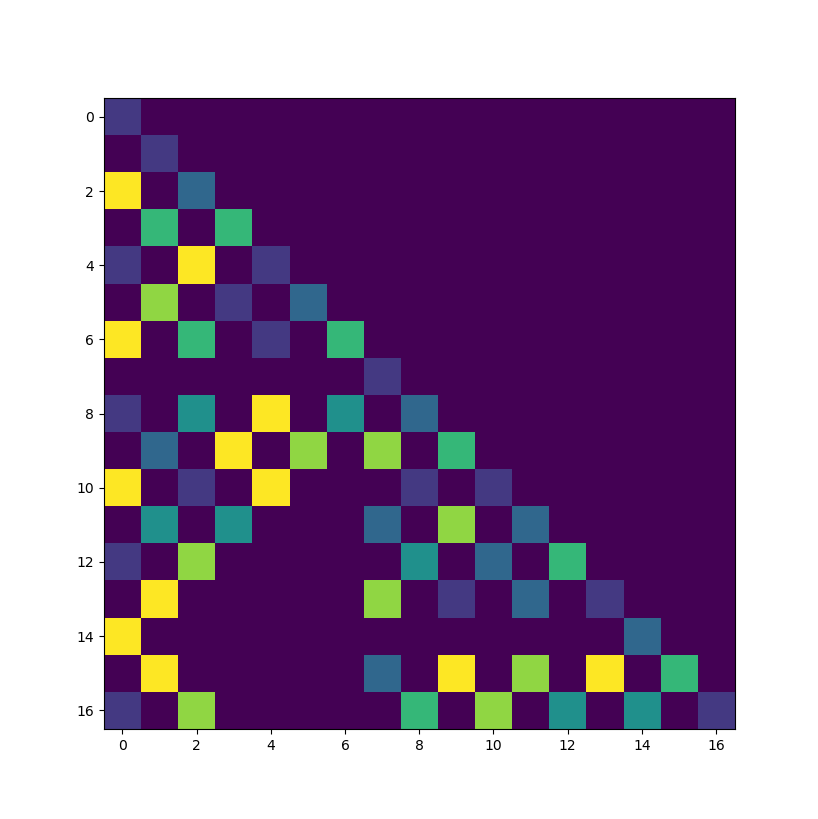
\includegraphics[scale=0.36]{16mod7.png}
 }
\end{frame}

\begin{frame}{$T_n(u)$ in $\mathbb{Z}_p[u]$}
 \center{What about more?}
\end{frame}

\begin{frame}{$T_n(u)$ in $\mathbb{Z}_p[u]$}
 \vspace{-18pt}
 \center{
  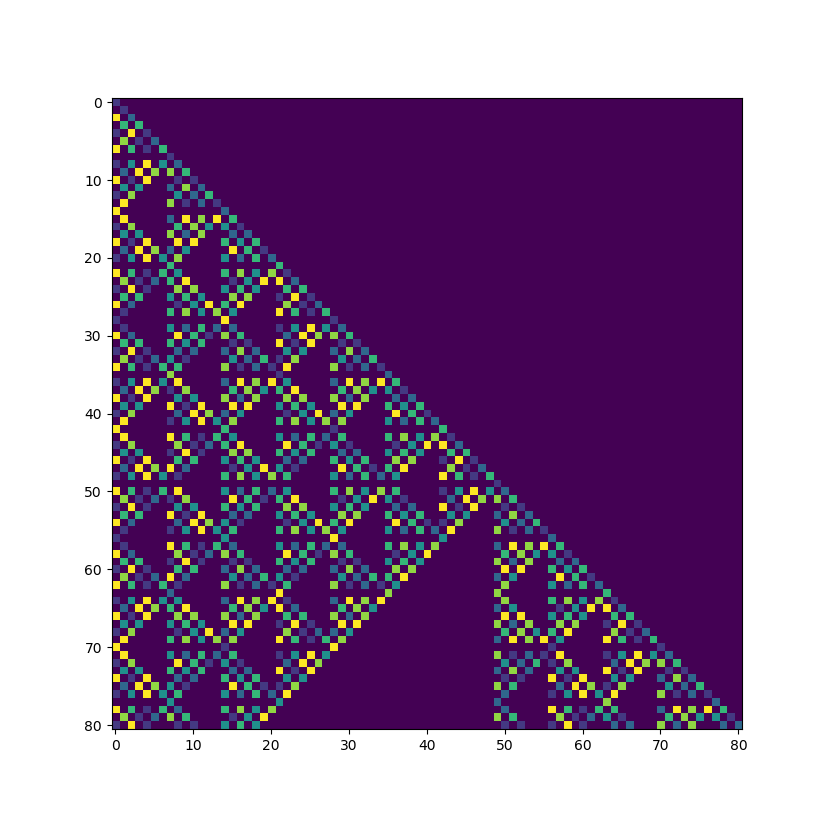
\includegraphics[scale=0.36]{80mod7.png}
 }
\end{frame}

\begin{frame}{$T_n(u)$ in $\mathbb{Z}_p[u]$}
 \center{Even more?}
\end{frame}

\begin{frame}{$T_n(u)$ in $\mathbb{Z}_p[u]$}
 \vspace{-18pt}
 \center{
  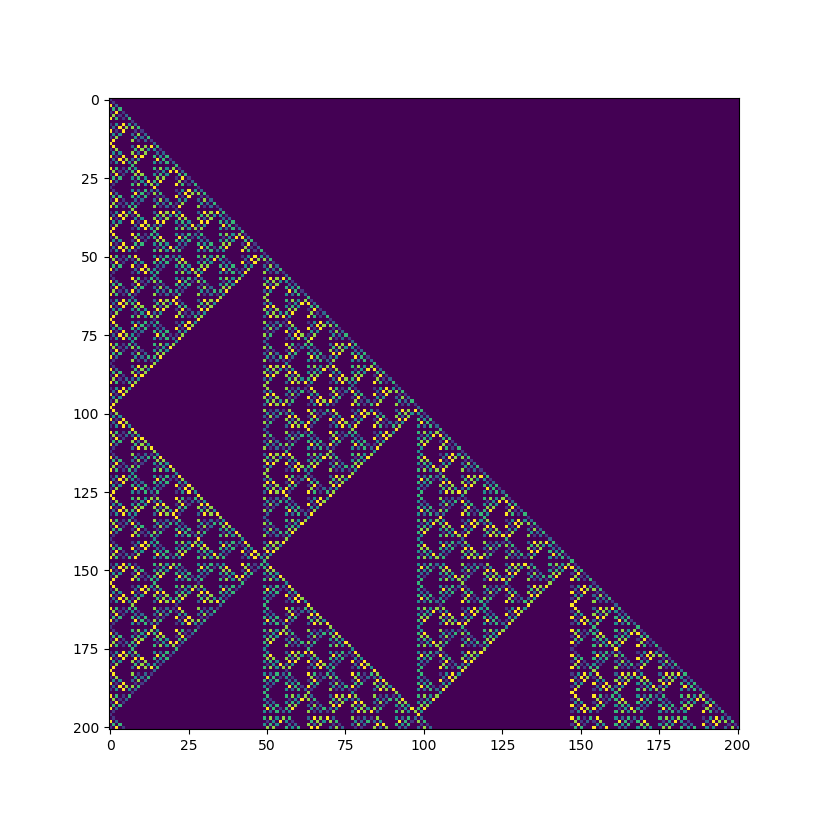
\includegraphics[scale=0.36]{200mod7.png}
 }
\end{frame}

\begin{frame}{$T_n(u)$ in $\mathbb{Z}_p[u]$}
 \center{What about some other primes $p$?}
\end{frame}

\begin{frame}{$T_n(u)$ in $\mathbb{Z}_p[u]$, $p=5$}
 \vspace{-18pt}
 \center{
  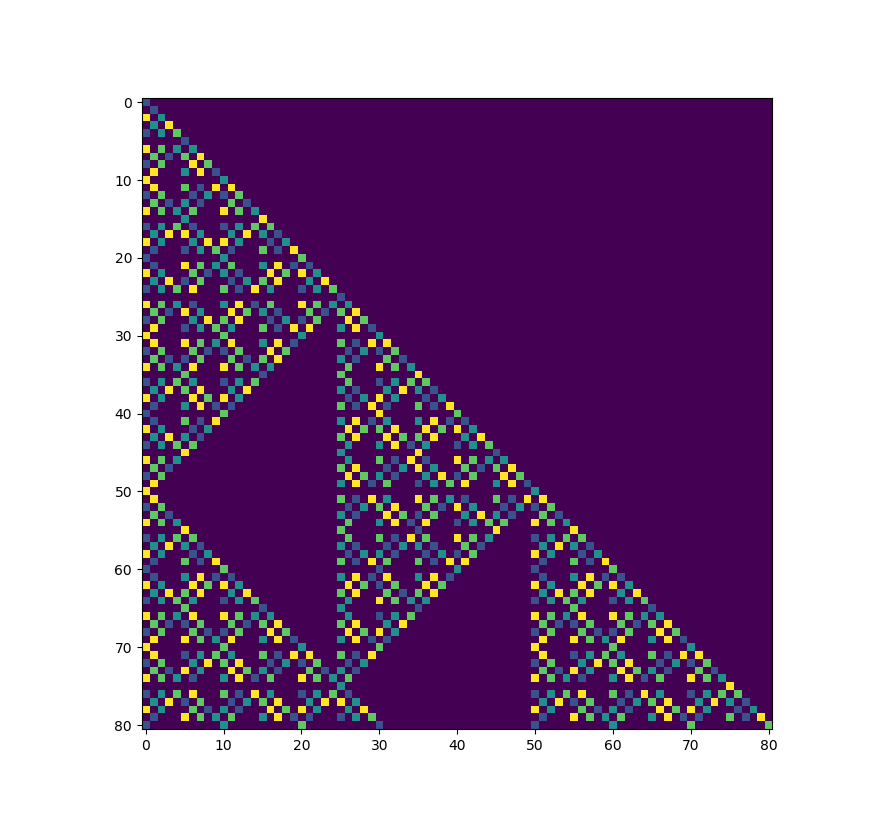
\includegraphics[scale=0.36]{80mod5.png}
 }
\end{frame}

\begin{frame}{$T_n(u)$ in $\mathbb{Z}_p[u]$, $p=11$}
 \vspace{-18pt}
 \center{
  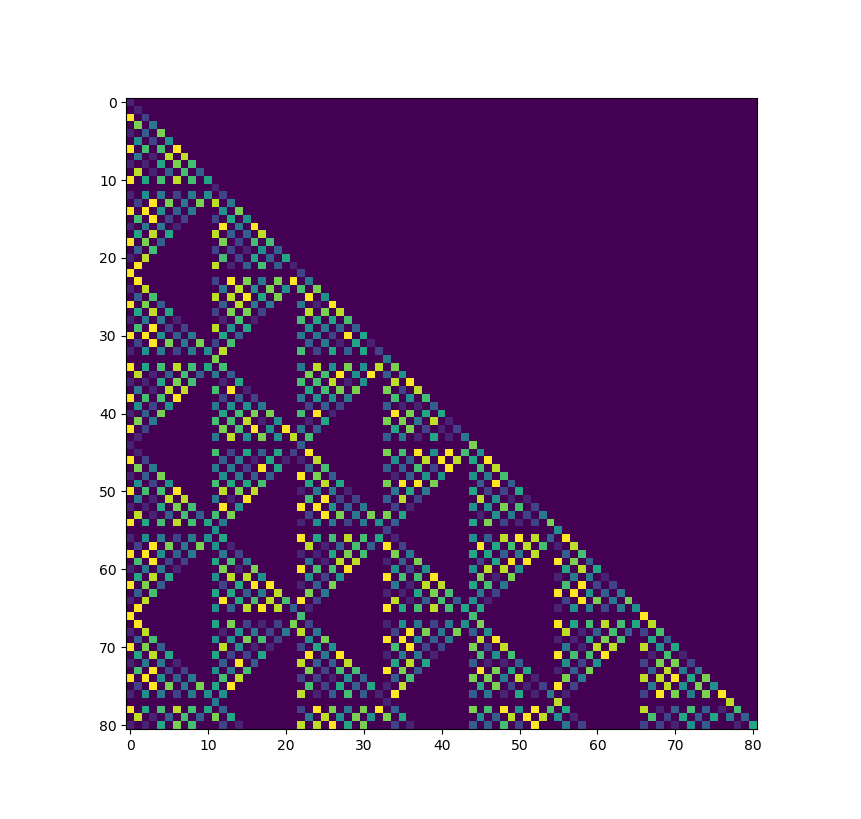
\includegraphics[scale=0.36]{80mod11.png}
 }
\end{frame}

\begin{frame}{$T_n(u)$ in $\mathbb{Z}_p[u]$, $p=3$}
 \vspace{-18pt}
 \center{
  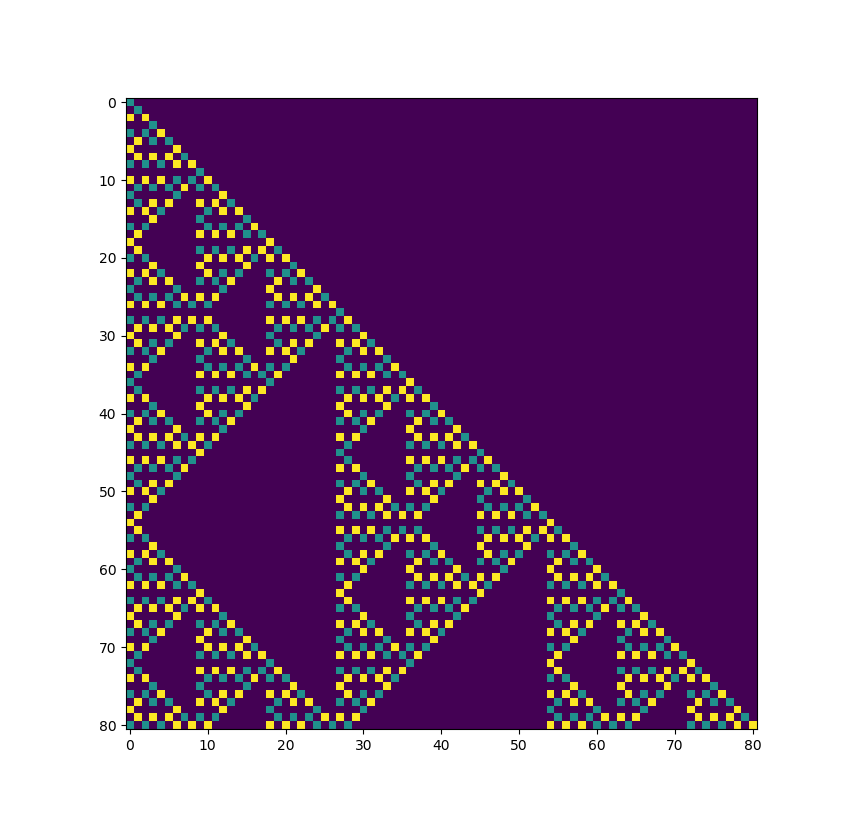
\includegraphics[scale=0.36]{80mod3.png}
 }
\end{frame}

\begin{frame}{$T_n(u)$ in $\mathbb{Z}_p[u]$, $p=3$}
 \vspace{-18pt}
 \center{
  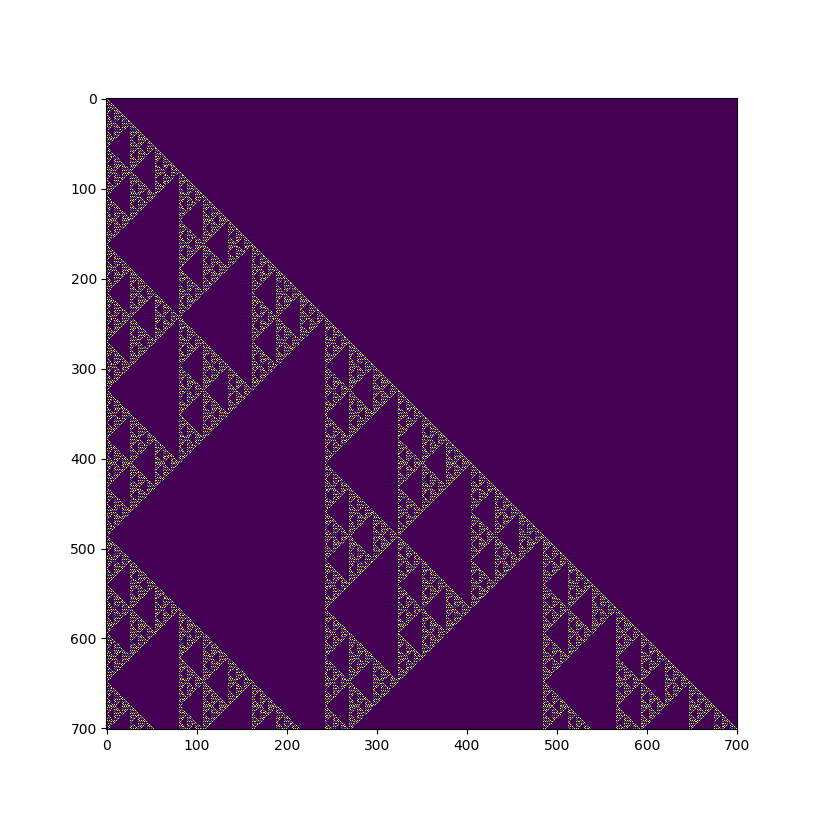
\includegraphics[scale=0.36]{700mod3.png}
 }
\end{frame}

\begin{frame}{What next?}
 \vspace{-18pt}
 \textbf{Continuations}
 \begin{itemize}
  \item Let $S_{n}(u)=\frac{\sin(nx)}{\sin{x}},\text{ where } u = \cos x$.
 \end{itemize}
 \begin{align*}
  S_{1} & = 1                      \\
  S_{2} & = 2u                     \\
  S_{3} & = 4u^{2} -1              \\
  S_{4} & = 8u^{3} - 4u            \\
  S_{5} & = 16u^{4} - 12u^{2} + 1  \\
  S_{6} & = 32u^{5} - 32u^{3} + 6u
 \end{align*}
 \center{We discover that similarly, $S_n(u)=2S_{n-1}(u)\cdot u - S_{n-2}(u)$}
\end{frame}

\begin{frame}{What next?}
 We also discover that\dots
 \begin{conjecture}
  \vspace{-12pt}
  \[n\in\mathbb{N} \text{ odd} \implies \sin(nx) = (-1)^{\frac{n-1}{2}}\cdot  T_{n}(\sin x)\]
 \end{conjecture}
 \begin{conjecture}
  \vspace{-12pt}
  \[n\in\mathbb{N} \text{ even} \implies \sin(nx) = (-1)^{\frac{n}{2}-1} \cdot \cos x \cdot S_{n}(\sin x)\]
 \end{conjecture}
\end{frame}

\begin{frame}{What next?}
\begin{itemize}
    \item Let $A_n(v)=\tan(nx)$, where $v=\tan(x)$. We have an explicit formula for this\dots
\end{itemize}
 \begin{conjecture}
  \vspace{-12pt}
  \[A_n(v) = \dfrac{\displaystyle\sum_{j=0}^{\left\lfloor \frac{n-1}{2} \right\rfloor} (-1)^j \cdot \binom{n}{2j + 1}\cdot v^{2j + 1}}{\displaystyle\sum_{j=0}^{\left\lfloor \frac{n}{2} \right\rfloor} (-1)^j \cdot \binom{n}{2j}\cdot v^{2j}}\]
 \end{conjecture}
\end{frame}

\begin{frame}{Thank You! \normalsize{(Panda per Arya's request)}}
 \center{
  
\includegraphics[scale=1.6]{panda.jpg}
 }
 \vspace{12pt}
\end{frame}

\end{document}
